%\documentclass[a4paper,9pt,fleqn,notoc]{diss}
%% \renewcommand{\includegraphics}[1][1]{} 
%\begin{document}

\chapter{Construction Grammar with FCG}
\label{s:fcg}
Construction Grammar posits that  linguistic
knowledge is organized in the form of \emph{constructions}  \citep{goldberg1995constructions,croft2001radical}\index{Goldberg, A.}\index{Croft, W.}
which are mappings of semantics and pragmatics to syntax, 
i.e. words and grammar, but also phonology, prosody or intonation. 
Typically, construction grammarians take a functional view on language
and analyze every piece of language as a tool for communication and 
in terms of the syntactic and semantic function it performs.
The theoretical framework of Construction Grammar
is important for this book, because it integrates 
semantics with syntax and opens up 
ways for understanding the acquisition and evolution
of language as a tool for solving communicative problems 
in which all elements of processing from semantics to
syntax can be used as a tool for solving these
problems. 

Every part of an utterance has meaning and a semantic function. The 
meaning of a lexical item is the reference to the category, prototype 
or concept that it refers to. Its function is how it is used both 
in the semantic structure underlying the phrase  and in the
syntactic structure of the phrase. The following two examples
include the word ``rot'' (red) but they use the word in completely 
different syntactic and semantic structures. 
\begin{enumerate}
\item ``der rote Block'' (the red block)
\item ``Rot ist eine Farbe'' (red is a color)
\end{enumerate}
In Example 1 ``rot'' (red) is used to modify the set of objects
denoted by the word ``Block'' (block) whereas in 2 the
statement is about the color itself. We can precisely capture 
these differences in semantic function using cognitive operations
and IRL (an structure for Example 1 can be found in Section \ref{s:irl}). 
The semantic function is coupled to a particular expression
in syntax. In Example 1 the color is expressed
as an adjective which signals its use as a modifier.  
In Example 2 the color is expressed as a noun and
signals that the subsequent verb phrase is a fact about the color itself. 
In production, the speaker can therefore choose to express
the category as an adjective if the category is linked to the corresponding
cognitive operation (e.g. {\footnotesize\tt apply-color}). In parsing, when
he observes a color adjective this allows him to infer
that he is supposed to modify a set of objects using that operation.
Which set of objects the color adjective modifies is determined
by the larger syntactic and semantic context. For instance, in Example
1 the adjective is part of an adjective noun phrase that 
indicates which set is modified by the color category namely
the set of blocks. From the viewpoint of the adjective noun phrase
the adjective has the semantic function of providing a modifier and in 
particular of modifying the set of objects denoted by the noun. Of course, other adjectives,
such as spatial adjectives can have the same function within an 
adjective noun phrase. The modified set is then input to another
operation namely the operation {\footnotesize\tt apply-selector}
which is marked by the determiner. So what we can see already in 
these simple examples are mappings 
from semantics to syntax and back, where every aspect of syntax,
i.e. words and grammatical relations
have a specific effect on the semantic interpretation of the phrase.
Vice versa, the speaker can use all the potential of syntax to
communicate precise semantic distinctions that he wants to convey.
The key item for analysis is the function of items 
both in syntax and semantics. 
These dependencies between syntax and semantics can be easily
operationalized using Fluid Construction Grammar (FCG) \index{Fluid Construction Grammar}
\citep{beule2005hierarchy,steels2005linking}\index{De Beule, J.}\index{Steels, L.}\index{Neubauer, N.}. 

Throughout this book language processing is implemented
in a computational implementation of Construction Grammar 
called Fluid Construction Grammar (FCG) . FCG is 1) a formalism
that provides a notation for specifying constructions, 2) a
an engine that processes linguistic structure by applying constructions, 
in order, to produce utterances or parse meanings, 3) a set of design principles
for organizing the grammar and linking grammar to 
representations of semantics, in particular, to semantic structure 
formalized using IRL. 

\section{Linguistic Processing}
Linguistic processing encompasses both production and parsing
of utterances. In production, FCG starts from a conceptualized
meaning and tries to translate as much as possible of
the semantic structure conceptualized by IRL into syntactic structure, 
i.e. words and grammatical relations using constructions in the linguistic inventory. 
In parsing this process is reversed and the construction inventory is used
to recover as much semantic structure from an utterance as possible.
Processing is organized around the \emph{transient structure}\index{transient structure}
which acts as a blackboard representing the current state of processing.
Constructions work like rules. If a construction is applicable,
i.e. if conditions for its application are met, the construction
can change the transient structure.
Over time the transient structure accumulates information provided by the different constructions
that have applied until some end state is reached, for instance,
no construction can apply anymore.

\begin{figure}
\begin{center}
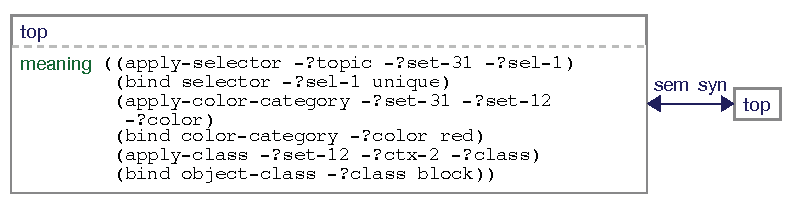
\includegraphics[width=1.0\columnwidth]{figs/simple-grammar-initial}
\end{center}
\caption[Initial transient structure]{\index{transient structure!initial}Initial transient structure which 
contains only the meaning 
to be expressed in the top-unit of the semantic pole (left).
There is no hierarchy yet and the syntactic pole (right) is empty.}
\label{f:initial-structure}
\end{figure}

\begin{sidewaysfigure}
\begin{center}
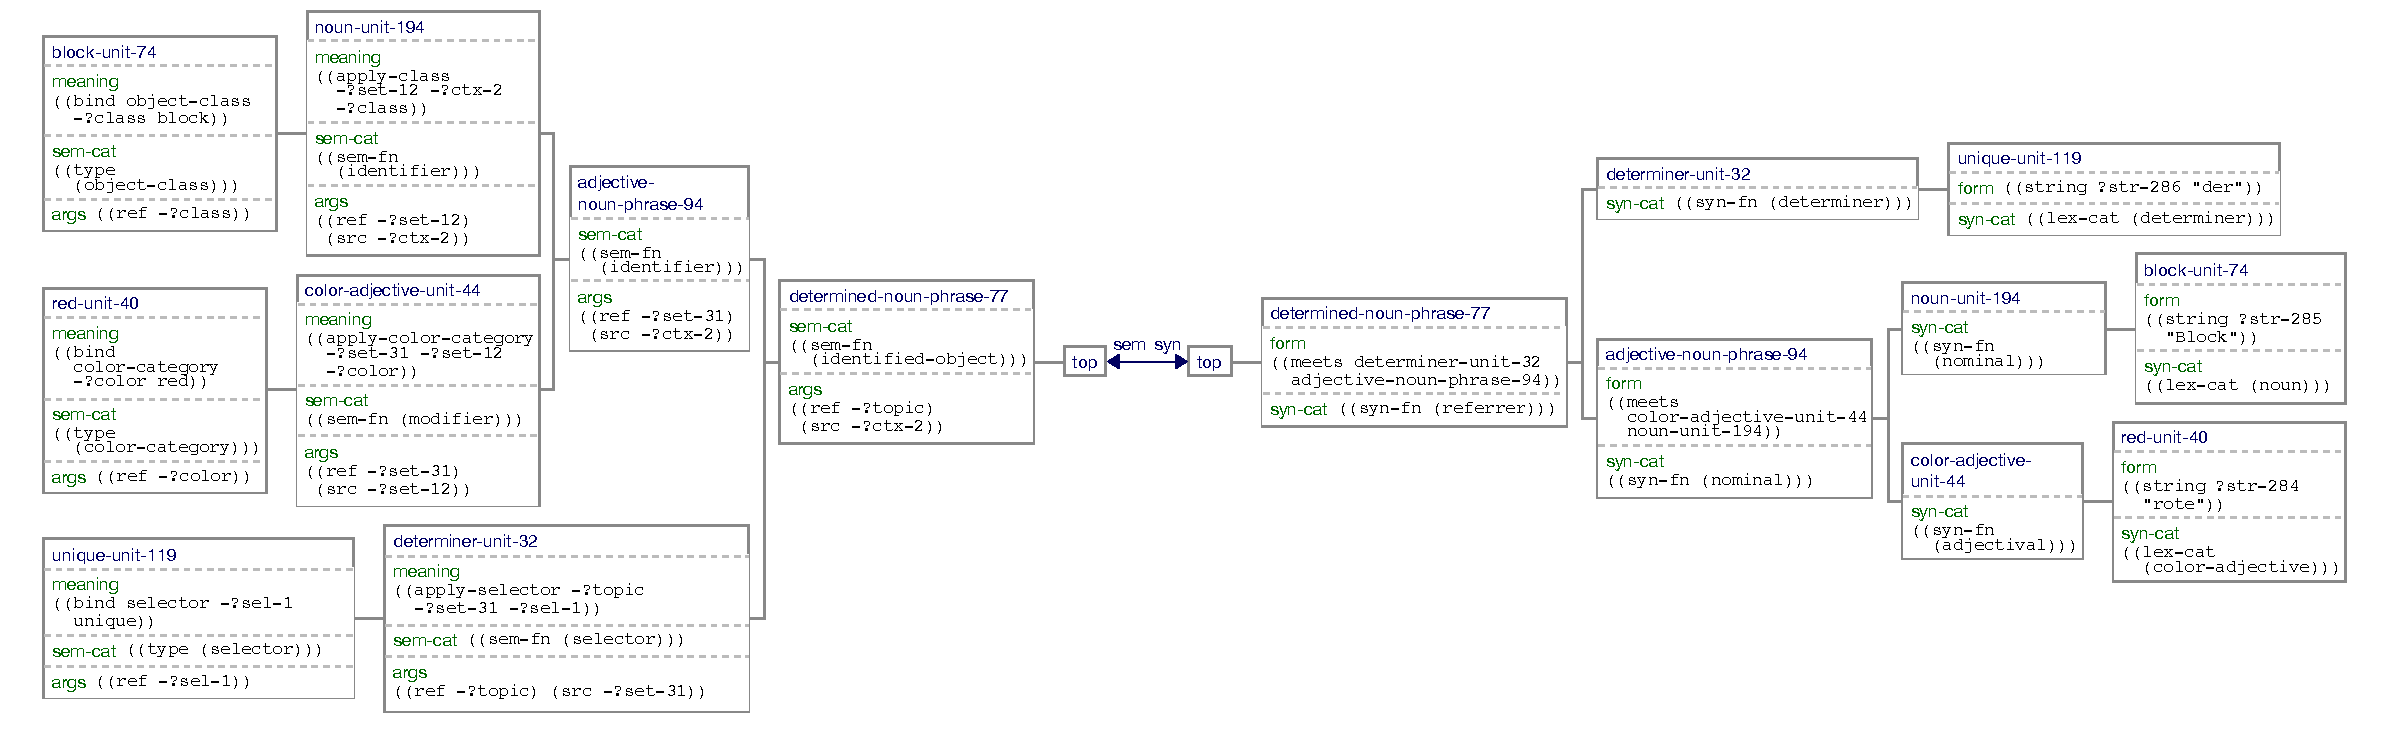
\includegraphics[width=1.0\columnwidth]{figs/simple-grammar-final}
\end{center}
\caption[Final transient structure]{\index{transient structure!final}Final transient structure after 
many constructions of a simplified German grammar have applied.
The structure consists of units which are hierarchically organized starting
from the top-unit. The meaning to be expressed is distributed over various 
units on the semantic side. Units feature 
semantic and syntactic categorization ({\footnotesize\tt sem-cat} and {\footnotesize\tt syn-cat})
which was build up in processing to organize constituent structure and
allow for high-level constructions to abstract from individual items.
On the syntactic side units have {\footnotesize\tt form} features consisting
of strings providing words and, so called  \emph{meets constraints} which introduce 
word order.}
\label{f:final-structure}
\end{sidewaysfigure}

\paragraph*{Transient structure}\index{transient structure}
The transient structure\index{transient structure} has two poles: a semantic and a syntactic pole.
Information regarding meaning is accumulated on the semantic
side, information about words and grammatical relations are
gathered on the syntactic side. Information is organized into 
units identified by a unit-name. Units consist of attribute-value pairs. 
In order to represent constituent structure, units can form hierarchies 
in which some units are hierarchically linked to other units effectively 
building tree like structures.
In the beginning of processing the transient structure\index{transient structure} is filled with 
information either from the conceptualization 
processes, e.g. in production, or from the utterance observed, e.g.
in parsing. Subsequently, constructions change the transient structure by adding new
units, introducing hierarchy, changing the value of attributes or by introducing 
new attributes. Figures \ref{f:initial-structure} and \ref{f:final-structure} show the transition from 
an initial transient structure\index{transient structure} which only contains a single unit, called \emph{top-unit} 
on each side to a final transient structure with hierarchical organization of units 
and many more features. The initial structure only contains a 
meaning on the semantic side. The final structure contains,
among other things, strings and syntactic word order constraints 
which can be used to build an utterance, a process called \emph{rendering}.
Figures \ref{f:initial-structure} and \ref{f:final-structure} show graphical representations
of the list representation (s-expression) used in processing. The
following restates the initial transient structure\index{transient structure} as s-expression.
\begin{footnotesize}
\begin{verbatim}
((top
  (meaning ((apply-selector -?topic -?set-31 -?sel-1)
            (bind selector -?sel-1 unique)
            (apply-color-category -?set-31 -?set-12 -?color)
            (bind color-category -?color red)
            (apply-class -?set-12 -?ctx-2 -?class)
            (bind object-class -?class block)))))
<-->
((top))
\end{verbatim}
\end{footnotesize}
The top shows the semantic pole. The bottom, after the {\footnotesize\tt <-->},
shows the syntactic pole. Both poles have one unit (the top-unit). 
On the semantic side the top-unit has one attribute, the meaning attribute
which has as its value an IRL-network in list form. 
The following shows the final structure in the same representational 
format.
\begin{footnotesize}
\begin{verbatim}
(...
 (color-adjective-unit-44
  (meaning ((apply-color-category -?set-31 -?set-12 -?color)))
  (sem-subunits (red-unit-40))
  (sem-cat ((sem-fn (modifier))))
  (args ((ref -?set-31) (src -?set-12))))
 (red-unit-40
  (meaning ((bind color-category -?color red)))
  (sem-cat ((type (color-category))))
  (args ((ref -?color))))
  ...
 (top (sem-subunits (determined-noun-phrase-77))))
<-->
(...
 (color-adjective-unit-44
  (syn-subunits (red-unit-40))
  (syn-cat ((syn-fn (adjectival)))))
 (red-unit-40
  (form ((string ?str-284 "rote")))
  (syn-cat ((lex-cat (color-adjective)))))
  ...
 (top (syn-subunits (determined-noun-phrase-77))))
\end{verbatim}
\end{footnotesize}
Only parts of the complete final structure are shown,
in particular, three units on each pole are shown the 
{\footnotesize\tt red-unit-40}, {\footnotesize\tt color-adjective-unit-44}
and {\footnotesize\tt top}. In contrast to the initial transient structure,
meaning is distributed across different units.
Notice that which unit is subunit of another is coded by a special
attribute called {\footnotesize\tt syn-subunits} on the syntactic pole
and {\footnotesize\tt sem-subunits} on the semantic pole. Compare
this with Figure \ref{f:after-red-cxn} which shows the hierarchy in the final 
structure. For example {\footnotesize\tt red-unit-40} is a subunit of 
{\footnotesize\tt color-adjective-unit-44}.

\begin{figure}
\begin{center}
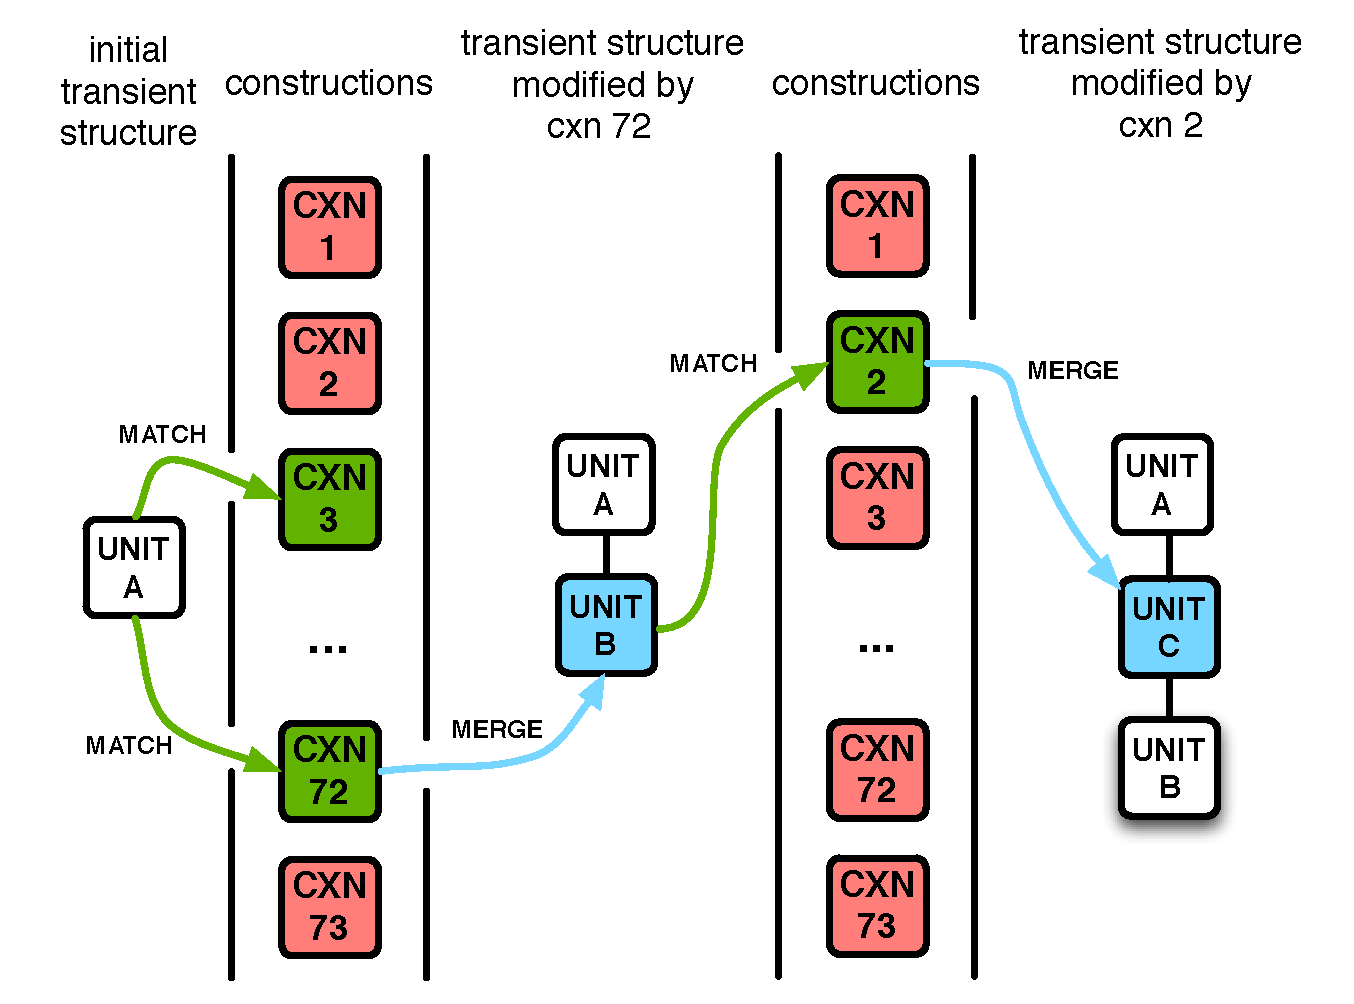
\includegraphics[width=0.8\columnwidth]{figs/high-level-cxn-application}
\end{center}
\caption[Construction application]{This figure shows a schematic view on 
construction application (Figure adapted from \citealp{steels2011design}\index{Steels, L.}).
Starting from the initial transient structure\index{transient structure} (left)
all constructions in the set of constructions are tested whether they 
match with the structure. Two constructions match with the
initial transient structure. If a construction matches it 
can merge new information. Construction 72 adds 
unit C. After the structure has been changed, the process continues
and all constructions are checked whether they merge with
the transient structure\index{transient structure} modified by construction 72.
Because construction 72 has applied, the transient
structure is in a state such that construction 2 can now apply. 
This was previously not the case. Construction 2 is depending on
information provided by construction 72. Subsequently, construction 2 
further changes the transient structure and so on and so forth.
Often multiple constructions from the set of constructions can apply.
For example, construction 3 could also change the initial transient structure\index{transient structure}.
This poses a general problem in processing which is solved
by using a search algorithm described later in this section.}
\label{f:cxn-application}
\end{figure}
\paragraph*{Constructions}\index{construction}
Constructions are organized in the same way as transient structures\index{transient structure}.
They consist of two poles and the data in each pole is organized in terms of units, 
attributes and values. FCG supports bi-directional constructions which means
that the same construction is used in production and parsing. 
The difference between production and parsing is how the syntactic and semantic 
pole of a construction is used in each case. 
In production the semantic pole is used to check the applicability
of the construction. In parsing the syntactic pole is used. Applicability
of a construction is checked using a mechanism called \emph{matching}.\index{matching}
Matching is based on the well studied concept of \emph{unification} which \index{unification}
is a computational process for equating two terms in this 
case the semantic or syntactic pole of the construction with the corresponding 
pole of the transient structure. If matching succeeds, the construction can
change both poles of the transient structure\index{transient structure}, a process called \emph{merge}
because it fuses information.
The precise inner workings of these two fundamental operations 
are described in \cite{steels2006fcg}\index{Steels, L.}\index{De Beule, J.}.
The most important fact is that matching in FCG mainly relies on 
variables, which in FCG (and in IRL) start with {\footnotesize\tt ?}.
In computational terms constructions specify 1) under which conditions
they apply and 2) if they apply how the structure should be changed.


\begin{figure}
\begin{center}
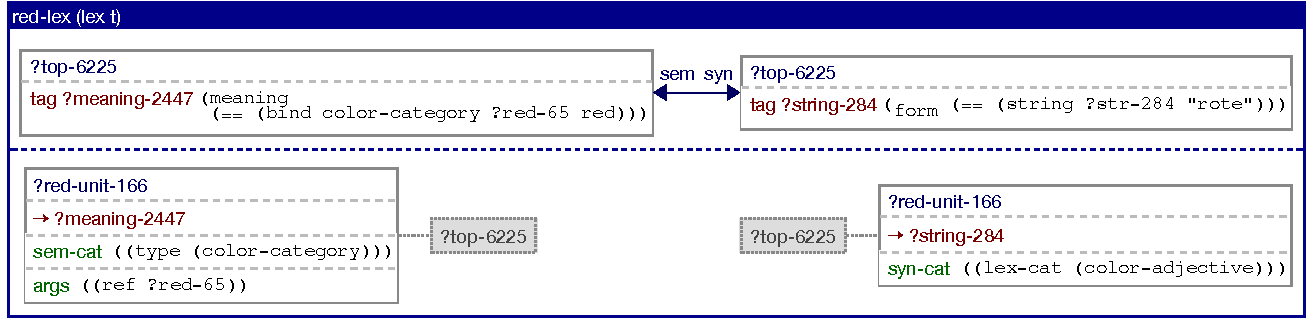
\includegraphics[width=1.0\columnwidth]{figs/lex-rot-cxn}
\end{center}
\caption[Schematic representation of a construction]{Schematic representation 
of a construction. The two poles
of the construction are shown. The top shows 
the tagged and matching parts of the construction. The 
bottom shows the hierarchy building part of the construction.}
\label{f:lex-rot-cxn}
\end{figure}

Figure \ref{f:lex-rot-cxn} shows an example of a lexical construction that maps 
the color category {\footnotesize\tt red} onto the string ``rote'' (red)
(Figure \ref{f:after-red-cxn} shows what happens
when this construction is applied to the initial transient structure\index{transient structure!initial}). 
The following shows the low-level list representation of the construction
schematically depicted in Figure \ref{f:lex-rot-cxn}
\begin{example}
\label{e:red-lex-list}
\begin{footnotesize}
\begin{Verbatim}[commandchars=\\\{\}]
((?top-6143
  (tag ?meaning-2381 
   (meaning (== (bind color-category ?red-57 red)))))
 ((j ?red-unit-158 ?top-6143)
  ?meaning-2381
  (sem-cat ((type (color-category))))
  (args ((ref ?red-57)))))
<-->
((?top-6143
  (tag ?string-251 (form (== (string ?str-251 "rote")))))
 ((j ?red-unit-158 ?top-6143)
  ?string-251
  (syn-cat ((lex-cat (color-adjective))))))
  \end{Verbatim}
\end{footnotesize}
\end{example}
The top displays the semantic pole followed by the syntactic pole after the 
{\footnotesize\tt <-->}. In production the construction requires\index{production}
the meaning {\footnotesize\tt (bind color-category ?red red)} to be present.
if this is the case the construction merges the information 
on the syntactic side, in particular, the stem into the transient structure\index{transient structure}.
Additionally, this construction builds hierarchy. It introduces a new unit
which is a subunit of the top-unit and which is used to collect
information for this particular lexical item. Already this simple 
construction uses the four basic ways in which constructions
interact with the transient structure\index{transient structure}. 
\begin{description}
\item[Variables and matching] Constructions inevitably contain
many variables. Already the unit names in the transient structure\index{transient structure}
are changing every time a new utterance is parsed or a new meaning
is produced. But also, just to give another example, variables in the meaning 
linking cognitive operations are different every time IRL conceptualizes. 
Using a variable in one part of the construction and repeating it in another 
can lead to changes in the transient structure triggered
by matching and merging \citep{steels2006fcg}\index{Steels, L.}\index{De Beule, J.}.
Example \ref{e:red-lex-list}, for instance, uses matching and merging
by re-using the variable in the meaning {\footnotesize\tt ?red-57}
in the {\footnotesize\tt args} attribute. Whatever this variable binds
to in processing the re-occurring variable will make sure
that the data is available in both places.
\item[Hierarchy] Hierarchy is built using a special
operator called the \emph{J-operator} which changes the
transient structure to include a new unit \citep{beule2005hierarchy}\index{De Beule, J.}\index{Steels, L.}.
The new unit can have units that are already present in the 
transient structure as children. A construction can therefore 
easily change the hierarchical structure of the complete pole.
The J-operator syntax is the following.
%\begin{example*}
%\label{e:j-op-syntax}
\begin{footnotesize}
\begin{Verbatim}[commandchars=\\\{\}]
((J ?new-unit ?parent (?child-1 .. ?child-n))
 (new-attribute new-attribute-value))
\end{Verbatim}
\end{footnotesize}
%\end{example*}
In the example construction the J-operator is used on the semantic
and on the syntactic side. It introduces new units on both sides 
and adds information to this unit (in Figure \ref{f:lex-rot-cxn}
the parts pertaining to the J-operator are shown below the dotted
line). Notice that the name of the new units is equal.
\item[Movement] Constructions can \emph{tag} attributes and
their values, in order, to move them around. In this example
construction the tag-operator moves the bind statement pertaining to the
color category from the top-unit to the newly created unit.
The tag operator takes the following form
\begin{footnotesize}
\begin{Verbatim}[commandchars=\\\{\}]
(?unit (tag ?tag-variable (attribute attribute-value))
\end{Verbatim}
\end{footnotesize}
The operator binds whatever follows the variable {\footnotesize\tt ?tag-variable}
to the variable. If the variable is used in a J-unit, i.e. a unit with a J-operator, 
in another part of the construction this denotes the place where 
{\footnotesize\tt (attribute attribute-value)} will be moved. The example
construction has tag operators on the semantic side for moving the
bind statement to the new semantic unit. Similarly, on the syntactic side the
operator is used to move the string ``rote'' to the new syntactic unit.
\end{description}

\begin{figure}
\begin{center}
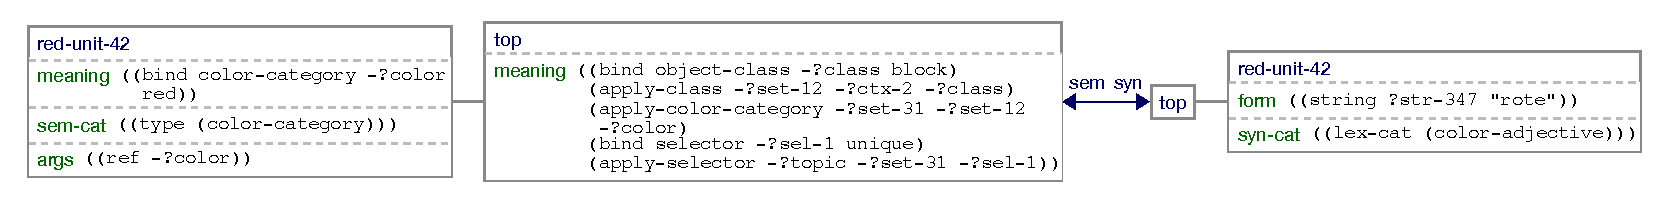
\includegraphics[width=1.0\columnwidth]{figs/simple-grammar-after-red-application}
\end{center}
\caption[Transient structure after lexical constructions applied]{
Transient structure after the lexical construction applied. The construction
has introduced two new units using the J-operator. 
One on the semantic side and one on the syntactic side.
Both units have the same name {\footnotesize\tt red-unit-42}. The construction introduced
the string ``rote'' on the syntactic side and the bind statements used for 
triggering the construction has been moved moved using the tag-operator 
from the top-unit to the new semantic subunit.
The construction also added new semantic and syntactic categories
({\footnotesize\tt sem-cat} and {\footnotesize\tt syn-cat}) that can be used by 
subsequent constructions.}
\label{f:after-red-cxn}
\end{figure}


\paragraph*{Search}
Constructions are organized in a pool of constructions. In
processing constructions, in principle, compete for access 
to the transient structure. Typically, more than one construction 
can apply to the transient structure and the question is how to organize
the process if there are multiple constructions that want to change
the transient structure. In the absence of apriori rules to 
prefer one construction over another, each construction that can 
apply to the transient structure\index{transient structure} is tried in a different branch of a 
heuristics guided search process. In other words, instead
of having competing constructions change the same transient
structure, the structure is copied and each potentially
applying construction is applied to a copy without necessarily 
influencing the other. Naturally, this leads to different
branches in processing in which each branch
computes a particular parsing or production result.
Search is represented using a search tree in which each
node contains a transient structure. The initial node 
contains the initial transient structure. Leaf nodes contain final structures.
The search process itself can be manipulated. 
For instance, it is possible to remove and refrain from processing 
duplicate nodes which contain the same transient structure\index{transient structure}
and the order of following a particular branch can be 
influenced by how successful one predicts the branch to be.
Figure \ref{f:fcg-search} shows an example search tree for 
production of the utterance ``der rote Block''.

\begin{figure}
\begin{center}

\includegraphics[width=1.0\columnwidth]{figs/der-rote-block-fcg-search}
\end{center}
\caption[FCG search tree in production]{FCG search tree which 
produces ``der rote Block'' given the IRL-network
shown in Figure \ref{f:the-red-block-network}.}
\label{f:fcg-search}
\end{figure}

\paragraph*{Design Layer}
In order to design grammars it has proven beneficial
to abstract away from the low level processing layer of FCG and 
add a representational layer that connects high level linguistic 
analysis with the processing engine of FCG.
The idea is to allow re-occurring problems in grammar design
to be solved using \emph{templates} without having
to resort and copy the code needed for describing a construction
in the basic list notation. Templates 
are a general mechanism for expressing \emph{design patterns}\index{design pattern},
i.e. solutions that can be re-used to deal with the
same problem occurring in different situations. For instance,
all grammars implement phrasal constructions. One 
of the main semantic functions of phrasal constructions 
is to introduce variable equalities for linking constituents.
A template encapsulates the solution to the problem 
of linking constituents in a way that the solution can be re-used in other
phrasal constructions of the same grammar, but ideally of
course also for phrasal constructions in other grammars.
Templates are defined similar to functions. They
have a name and a set of arguments which are specific
to the template.
\begin{example}
\label{e:template-syntax}
\begin{footnotesize}
\begin{Verbatim}[commandchars=\\\{\}]
(\emph{template-name} \emph{construction-name}
 \emph{:argument-1} \emph{value-1}
 \emph{:argument-2} \emph{value-2}
 ...
 \emph{:argument-n} \emph{value-n})
\end{Verbatim}
\end{footnotesize}
\end{example}


Let us consider an example. I redefine the lexical construction introduced earlier,
using a template called 
{\footnotesize\tt def-lex-skeleton}.
\begin{example}
\label{e:def-lex-rot}
\begin{footnotesize}
\begin{Verbatim}[commandchars=\\\{\}]
(def-lex-skeleton red-cxn 
 :meaning (== (bind color-category ?cat red)) 
 :args ((ref ?cat))
 :string "rote")
\end{Verbatim}
\end{footnotesize}
\end{example}
If this template is executed it translates into the 
low-level list representation in Example \ref{e:red-lex-list}. 

\section{Open-ended Language Evolution with FCG}
Besides the obvious fact that one needs a computational
formalism for linguistic processing in order to do computational
experiments, FCG has a number
of features that make it an optimal choice for studies
in language evolution. FCG is not fixed to a certain
set of constructions, a particular grammar layout, 
a particular set of meanings,
or even a particular set of semantic and syntactic 
categories. FCG solely provides 
dedicated mechanisms for processing language but
makes no actual claims about how a particular
phenomenon in language should be processed. 
Most importantly it makes no claims about the 
layout of the constructions designed to process
a particular phenomenon. This allows different 
solutions to be explored by grammar designers.
But, more importantly, it allows artificial agents
to invent different constructions for solving a particular
problem in communication, track their success and
adapt them until the agents have conventionalized
a solution to their particular problem. This is a point
of utmost importance. Language is not a fixed system, but
rather a system negotiated by its users to reach
communicative goals in a decentralized manner. 
The fact that there are different solutions to solving
the same problem, therefore, requires formalisms
that are designed to be open to changing syntactic and 
semantic categorization, evolving meaning
structure and new constructions. FCG is such a formalism.

From a computational perspective, FCG provides
an easily manipulatable data representation which makes 
inventing new constructions, changing and
adapting semantic and syntactic categories,
introducing hierarchy or movement of data relatively easy.
In line with construction grammar the \emph{unified} nature
of representation is important. There is absolutely
no difference in terms of representation and processing 
between lexical, functional or phrasal constructions. Hence, FCG
supports research into how constructions can change 
from lexical to grammatical constructions, which is 
of interest for the study of the influence of grammaticalization 
processes on language evolution\citep{traugott1991grammaticalization}\index{Heine, B.}\index{Traugott, E. C.}.

Another important argument for the use of FCG is its robust
behavior in parsing and production. The search process\index{parsing}
for construction application and the bi-directional 
nature of constructions allow agents to produce
as much of the meaning as they can when they
are speaker. In parsing, the same process
allows agents to  recover as much of the semantics 
of a phrase as they possibly can. This is a prerequisite 
for any kind of grounded language learning let alone
language evolution. Agents have to get as much
information as possible from the different systems
such as perception and conceptualization, but also
language processing. If agents would have to deal with
a grammar engine that essentially gives up on processing
as soon as an agent encounters a phrase that he
thinks is unconventional, learning the new unconventional
phrase can never occur or is significantly hindered. Whereas
if the grammar engine provides as much information as 
possible agents have a much better shot at guessing
underlying meaning and making sense
of what was conveyed to them. Subsequently,
they can better represent the new parts of an 
utterance versus parts they already know.
Modeling this whole process as a search
process is an immense advantage of FCG.
Agents can track what changes when they
apply other constructions and explore different
possible parse and produce results, in order,
to identify problems in language processing.

The last point with respect to the advantage of
keeping information from the search process that
governs linguistic processing is important, in particular,
for the main problem studied in this book: conventionalization.
In order, for agents to realize that constructions are competing
for the same string, the same grammatical structure or
the same meaning, it is vital to fully explore the search process.
If there are multiple ways of producing an utterance for a meaning,
for instance, because there are multiple words to express
the same category, then the search can recover 
all of them. Together with a mechanism for tracking
success of constructions, the search can choose
the best one of them. After the interaction the agent can
then update the constructions used and those that
he could have used, for instance, by rewarding
successfully used constructions and punishing 
unsuccessful or unused constructions.
Constructions are equipped with a score that
allows agents to update their inventories
by scoring constructions according to their success
in communication. If scores get too low agents can remove
the affected constructions.

\section{Discussion}
There is no question that this is a short, in many ways too short,
introduction to FCG. FCG has been under continuous development
since 1998 and it has developed into a mature system which allows to 
to research complex language phenomena such as Russian aspect 
\citep{gerasymova2010acquisition,gerasymova2012temporal}\index{Gerasymova, K.}\index{Spranger, M.}. The complexity of natural 
language has no doubt left its mark on the system and many design 
choices in the system are not immediately obvious,
unless one takes the scope of the research program into account.
Recently several book projects \citep{steels2011design,steels2012computational}\index{Steels, L.}
attempted to communicate the full scope of FCG research
performed in the last 5-10 years. The interested reader is referred
to these efforts to get a broader introduction.

%\bibliographystyle{diss}
%\bibliography{papers,space} 
%\end{document}


